% =============================
% ภาคผนวก
% =============================
% หมายเหตุ: ก่อนเริ่มภาคผนวก ระบบจะสร้างหน้าคั่นให้อัตโนมัติ
% ใช้คำสั่ง \appendiceschapter{ชื่อภาคผนวก} สำหรับแต่ละภาคผนวก
% ระบบจะกำหนดตัวอักษร ก, ข, ค ... ให้โดยอัตโนมัติ
%
% *** ลบข้อความตัวอย่างด้านล่าง แล้วใส่ภาพ UI / Prototype ของตนเอง ***

% =============================
% ภาคผนวก ก
% =============================
\setcounter{chapter}{-1}
\appendiceschapter{ตัวอย่าง UI หรือ Prototype}

\section*{ภาพหน้าจอระบบ}

ภาคผนวกนี้แสดงตัวอย่างหน้าจอของระบบที่พัฒนาขึ้น เพื่อให้เห็นภาพรวมของการออกแบบส่วนติดต่อกับผู้ใช้

หน้าจอเข้าสู่ระบบ (Login) แสดงดังภาพที่ \ref{fig:ui_login}

% *** เปลี่ยนชื่อไฟล์จาก ui-login.png เป็นชื่อไฟล์ของคุณ ***
\begin{figure}[H]
\centering
% 
\includegraphics[width=0.8\textwidth]{images/ui-login.png}
\fbox{\parbox{0.75\textwidth}{\centering\vspace{4cm}\textit{แทรกภาพหน้าจอ Login ที่นี่}\\ใช้คำสั่ง \texttt{\textbackslash includegraphics}\vspace{4cm}}}
\caption{หน้าจอเข้าสู่ระบบ (Login)}
\label{fig:ui_login}
\end{figure}

หน้าจอหลัก (Dashboard) แสดงดังภาพที่ \ref{fig:ui_dashboard}

\begin{figure}[H]
\centering
% 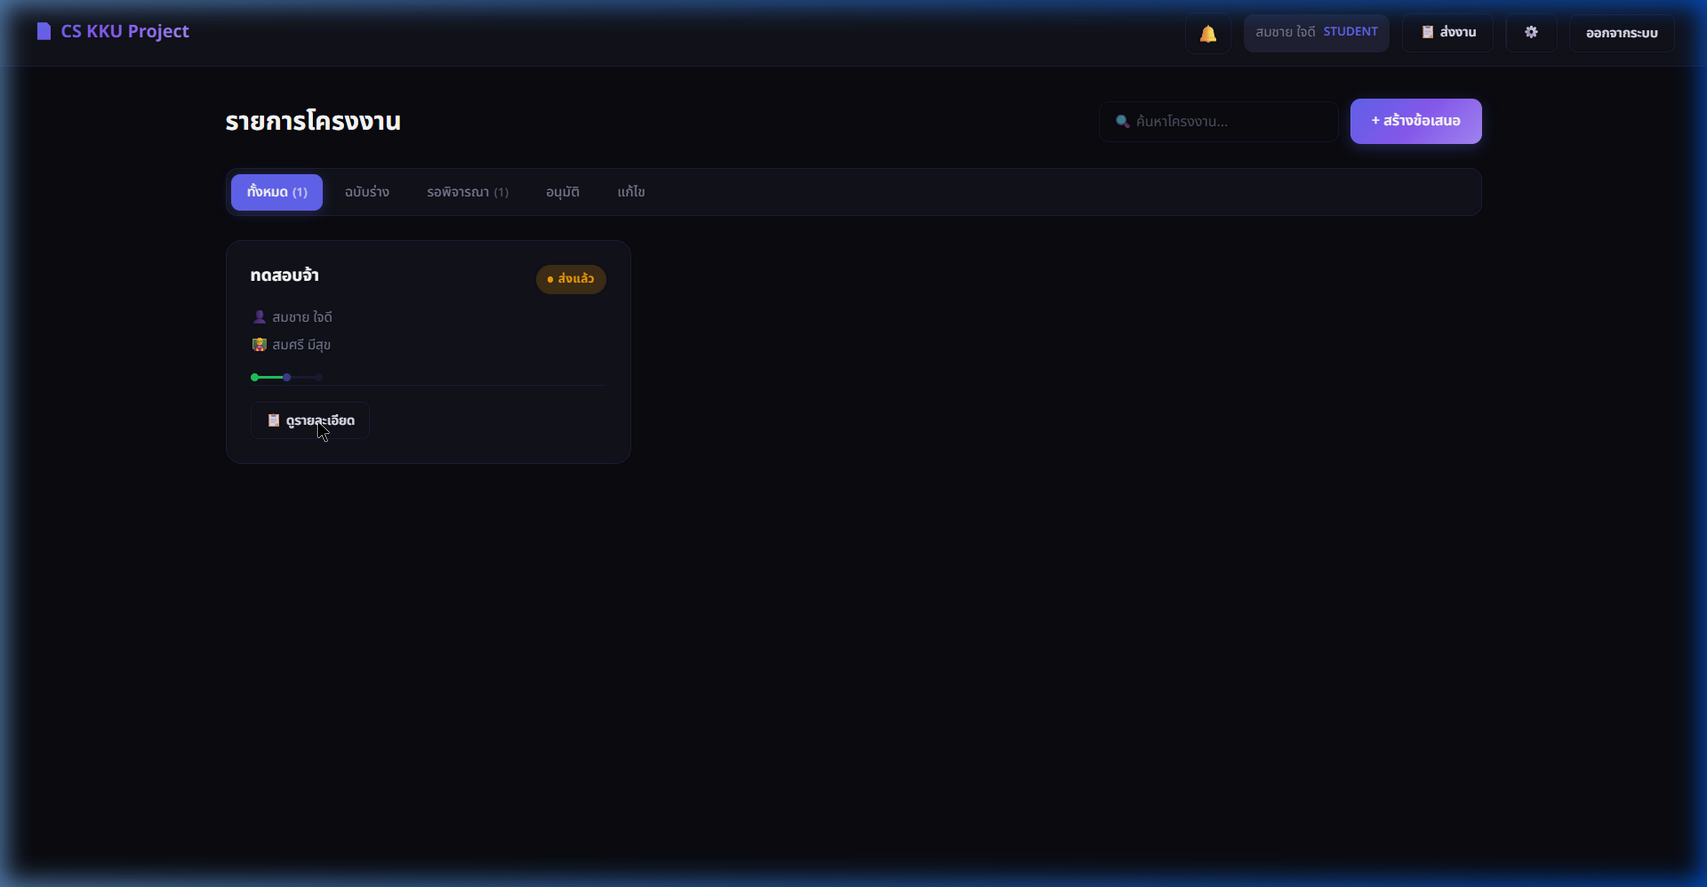
\includegraphics[width=0.8\textwidth]{images/ui-dashboard.png}
\fbox{\parbox{0.75\textwidth}{\centering\vspace{4cm}\textit{แทรกภาพหน้าจอหลักที่นี่}\vspace{4cm}}}
\caption{หน้าจอหลัก (Dashboard)}
\label{fig:ui_dashboard}
\end{figure}

\section*{คู่มือการใช้งาน}

อธิบายขั้นตอนการใช้งานระบบโดยสังเขป\ldots{}

% =============================
% ภาคผนวก ข
% =============================
\appendiceschapter{ความไวของพารามิเตอร์ Elo}

\section*{วิธีการ}

ค่า $K$ (ขนาดการปรับ) และ $h$ (ความได้เปรียบของเจ้าบ้าน) ของระบบ Elo ในหัวข้อการคำนวณคะแนน Elo ถูกเลือกบนข้อมูลที่อยู่ก่อนข้อมูลที่ใช้ฝึกและทดสอบแบบจำลองทั้งหมด ภาคผนวกนี้ทำการค้นหาซ้ำเพื่อให้ตรวจสอบได้ ดังนี้

\begin{enumerate}[label=\arabic*)]
    \item ใช้ผลการแข่งขันลีกของ 5 ลีกใหญ่จาก Football-Data.co.uk ฤดูกาล 2000--2001 ถึง 2014--2015 รวม 26,946 นัด โดยฤดูกาล 2000--2001 ถึง 2004--2005 ใช้เพียงอุ่นคะแนน Elo ให้เข้าที่
    \item คำนวณ Elo ใหม่สำหรับทุกคู่ $K \in \{5, 10, 15, 20, 25, 30\}$ และ $h \in \{0, 20, 40, 60, 80, 100\}$
    \item ทำนายผล H/D/A ด้วยแบบจำลองจำนวนประตู Poisson ที่ใช้ผลต่าง Elo เป็นตัวแปรเดียว แบบ Walk-forward บนฤดูกาล 2005--2006 ถึง 2014--2015 (18,260 นัด) โดยแต่ละฤดูกาลทำนายจากแบบจำลองที่ฝึกด้วยฤดูกาลก่อนหน้าเท่านั้น
\end{enumerate}

ผลสร้างซ้ำได้ด้วยคำสั่ง \texttt{uv run elo\_sensitivity}

\section*{ผลการทดสอบ}

\begin{table}[H]
\centering
\caption{Walk-forward Log Loss ฤดูกาล 2005--2006 ถึง 2014--2015 ตามค่า $K$ (แถว) และ $h$ (คอลัมน์) ตัวหนาคือค่าที่ใช้ในโครงงาน}
\label{tab:elo_sensitivity}
\begin{tabular}{|c|c|c|c|c|c|c|}
\hline
$K$ \textbackslash{} $h$ & 0 & 20 & 40 & 60 & 80 & 100 \\
\hline
5 & $0.9972$ & $0.9972$ & $0.9973$ & $0.9975$ & $0.9976$ & $0.9978$ \\
10 & $0.9942$ & $0.9942$ & $0.9943$ & $0.9943$ & $0.9944$ & $0.9945$ \\
15 & $0.9941$ & $0.9941$ & $\textbf{0.9941}$ & $0.9942$ & $0.9942$ & $0.9942$ \\
20 & $0.9950$ & $0.9950$ & $0.9950$ & $0.9950$ & $0.9950$ & $0.9949$ \\
25 & $0.9962$ & $0.9962$ & $0.9962$ & $0.9962$ & $0.9961$ & $0.9960$ \\
30 & $0.9976$ & $0.9976$ & $0.9976$ & $0.9975$ & $0.9975$ & $0.9973$ \\
\hline
\end{tabular}
\end{table}

ค่าที่ใช้ ($K = 15$, $h = 40$) ให้ Log Loss $0.9941$ เท่ากับค่าต่ำสุดของตาราง ค่า $h$ แทบไม่มีผล (ต่างกันไม่เกิน $0.0001$ ในแถว $K = 15$) เนื่องจากแบบจำลองจำนวนประตูเรียนรู้ความได้เปรียบของเจ้าบ้านจากค่าคงที่ของตัวเองอยู่แล้ว ส่วน $K$ ระหว่าง 10--20 ให้ผลต่างกันไม่เกิน $0.001$ และแย่ลงเมื่อ $K$ เล็กเกินไป (คะแนนปรับตัวช้า) หรือใหญ่เกินไป (คะแนนแกว่งตามผลนัดล่าสุด) การดึงคะแนนกลับสู่ค่าเฉลี่ยตอนต้นฤดูกาล (Season Regression) ร้อยละ 10, 20 และ 30 ให้ Log Loss $0.9944$, $0.9950$ และ $0.9958$ ตามลำดับ จึงไม่ได้ใช้

ผลนี้แสดงว่าข้อสรุปของโครงงานไม่ได้ขึ้นกับการเลือกค่าพารามิเตอร์ Elo ที่พอดีกับข้อมูล
